%\ihead{\headmark}
\chapter{Visualization and System Architecture}


\makeatletter
\renewcommand{\@chapapp}{}% Not necessary...
\newenvironment{chapquote}[2][2em]
{\setlength{\@tempdima}{#1}%
	\def\chapquote@author{#2}%
	\parshape 1 \@tempdima \dimexpr\textwidth-2\@tempdima\relax%
	\itshape}

\makeatother

\begin{center}
	\begin{chapquote}{}
		``A picture is worth a thousands words.''
	\end{chapquote}
\end{center}

Visualization allows us to see the broader aspects of complex data by showing the data in graphical formats \cite{quora:Sulakshana}. The visualization tool by Grafana has been used for displaying the real-time data received from the sensors. All devices send the data in real-time, which first store in InfluxDB and then Grafana tool loads those data and display it in a graphical format. 

\section{Grafana}
Grafana is an open source real-time visualization tool for analytics and monitoring. It is one of the best tools for time series analytics. Therefore, it has been used for visualizing the real-time data from sensor devices. It can be used for any kind of analytical application, for example, industrial sensors, home automation, hospitals, and weather reports. It can connect to many data sources and pull data from there for further analysis and the visualization. The most commonly used data sources these days are: Elasticsearch, InfluxDB, Graphite, Prometheus.


It allows us to connect these data sources easily, which makes it very convenient. Multiple dashboards can be created in Grafana in order to view different dimensions of the data. It also provides multiple tools for creating graphs in different fashions and styles, which can be simply added to dashboards.

\section{InfluxDB}
Since the sensor data is time critical. Therefore, a time series database is required for storing the data. InfluxDB is one of the best time series databases available. Therefore, it is chosen for storing the sensors data.

It is very easy to install and manage and does not require other dependencies to run. It also provides HTTP/HTPPS interface in order to read and write data from the database. The retention policy can be set on the database to manage space conveniently. The basic terms in InfluxDB are:

\begin{itemize}
	\item Database name
	\item Measurement (same as table name in traditional databases)
	\item Tags (to filter data)
	\item Fields (actual data values)
\end{itemize}

The fields are generally used as a key-value pair, with a timestamp field. Only one point can be stored at any specific timestamp. The precision of a single field can be set in second, in millisecond and even in nanosecond. If the field does not contain a timestamp field, then the InfluxDB will generate a timestamp automatically. Another reason for choosing the InfluxDB is that it is really easy to configure Grafana for using InfluxDB as a data source. 


\section{Setting up Grafana with InfluxDB}
The setup can be quickly done. Before starting, a database should be set up on InfluxDB. Once the database is ready, the Grafana server needs to start. Generally, it runs on port 3000 but because of ports conflict, it is recommended to change the port to some other address by editing the \textit{$conf/sample.ini$} file.


Once the server is started, browse \textit{localhost:3000} to open the Grafana web interface. Select an option to add a new data source and configure the InfluxDB data source as shown in Figure \ref{fig:gr_db_setup}. A database name, an IP address where the database is running, a username and a password are required to set it up.

\begin{figure}[htpb]
	\centering
	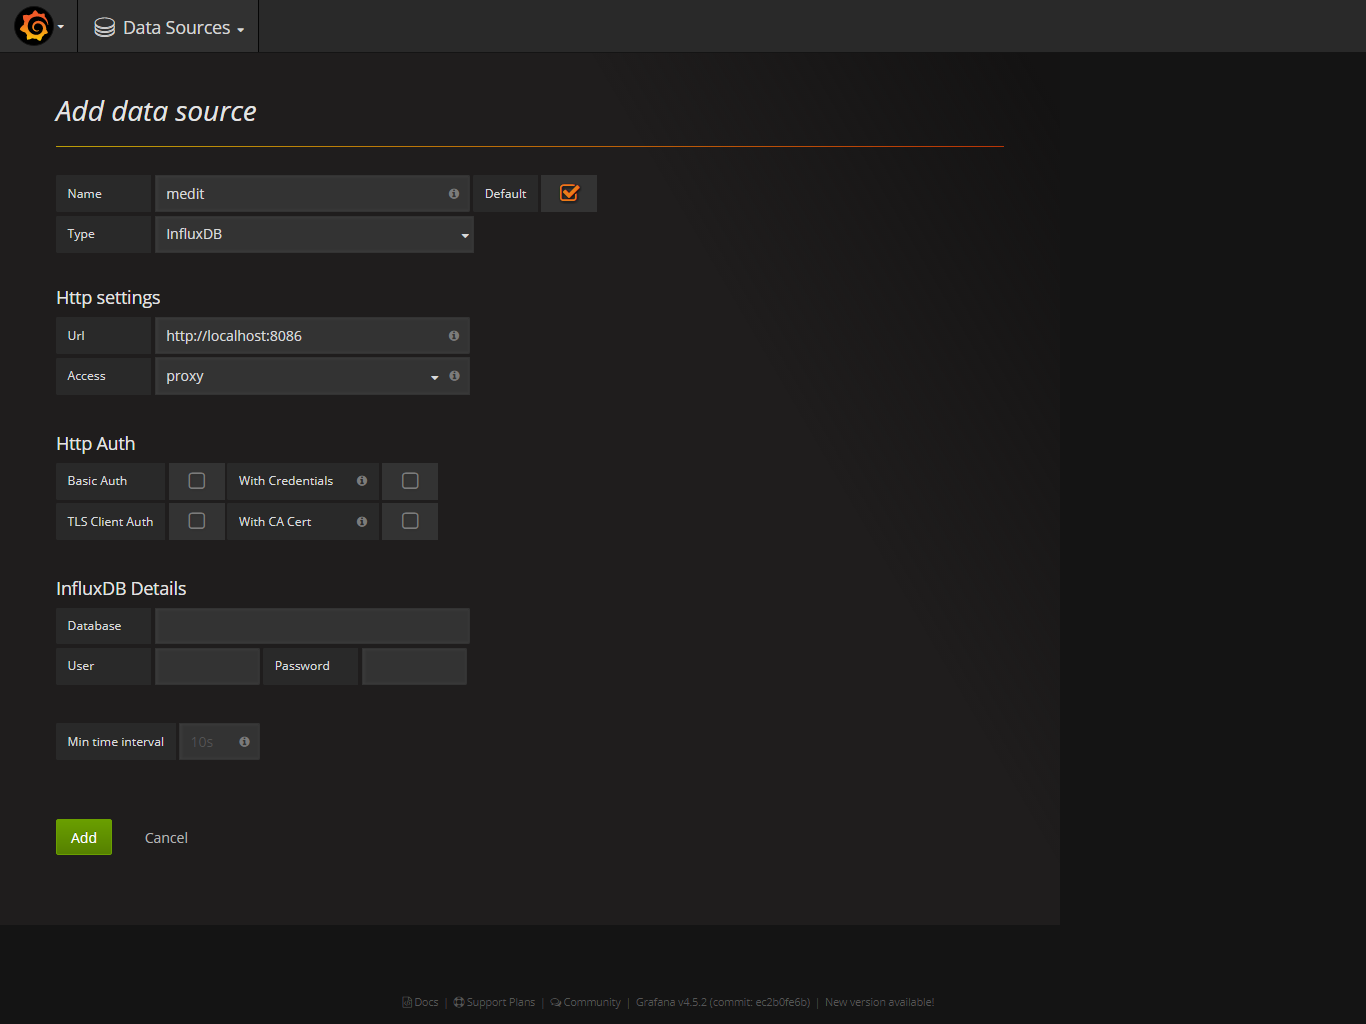
\includegraphics[width=16cm,height=15cm,keepaspectratio=true]{images/gr_db_setup}
	\caption{
		InfluxDB data source setup in Grafana.
	}
	\label{fig:gr_db_setup}
\end{figure}



\begin{figure}[htpb]
	\centering
	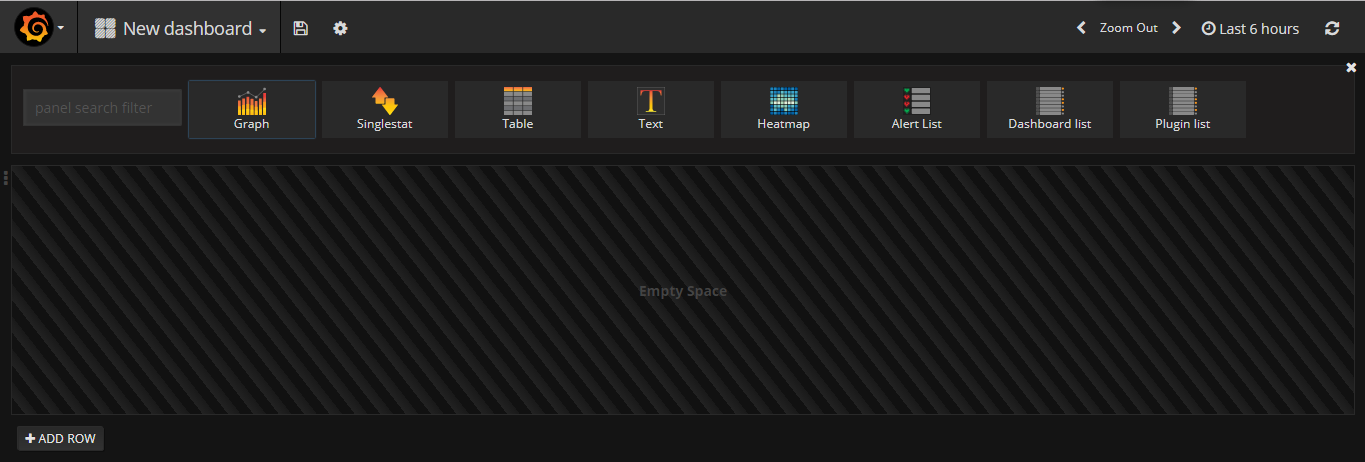
\includegraphics[width=16cm,height=15cm,keepaspectratio=true]{images/dashboard}
	\caption{
		Dashboard setup.
	}
	\label{fig:dashboard}
\end{figure}

Once the data source is set up, a dashboard is created to add the graphs and panels where the data can be visualized. Multiple types of panels are available by default such as table, graphs, text, single stat and alert list.

When a graph is added to a dashboard, a data source is needed to be defined for that graph. This can be done by selecting the graph and editing. The interface for setting up the data source can be seen in Figure \ref{fig:gr_query}. A user-friendly interface is available where one can define a query for the graph. A query can be built just by selecting the option from a drop down menu. It will contain all the information from the database that is set up in the data source, shown in Figure \ref{fig:gr_db_setup}. A user simply needs to select the data source, then select the specific measurement. One measurement can have multiple fields, therefore, select a specific required field. Once all the steps are done, the panel is ready to display the information from InfluxDB database.


\begin{figure}[htpb]
	\centering
	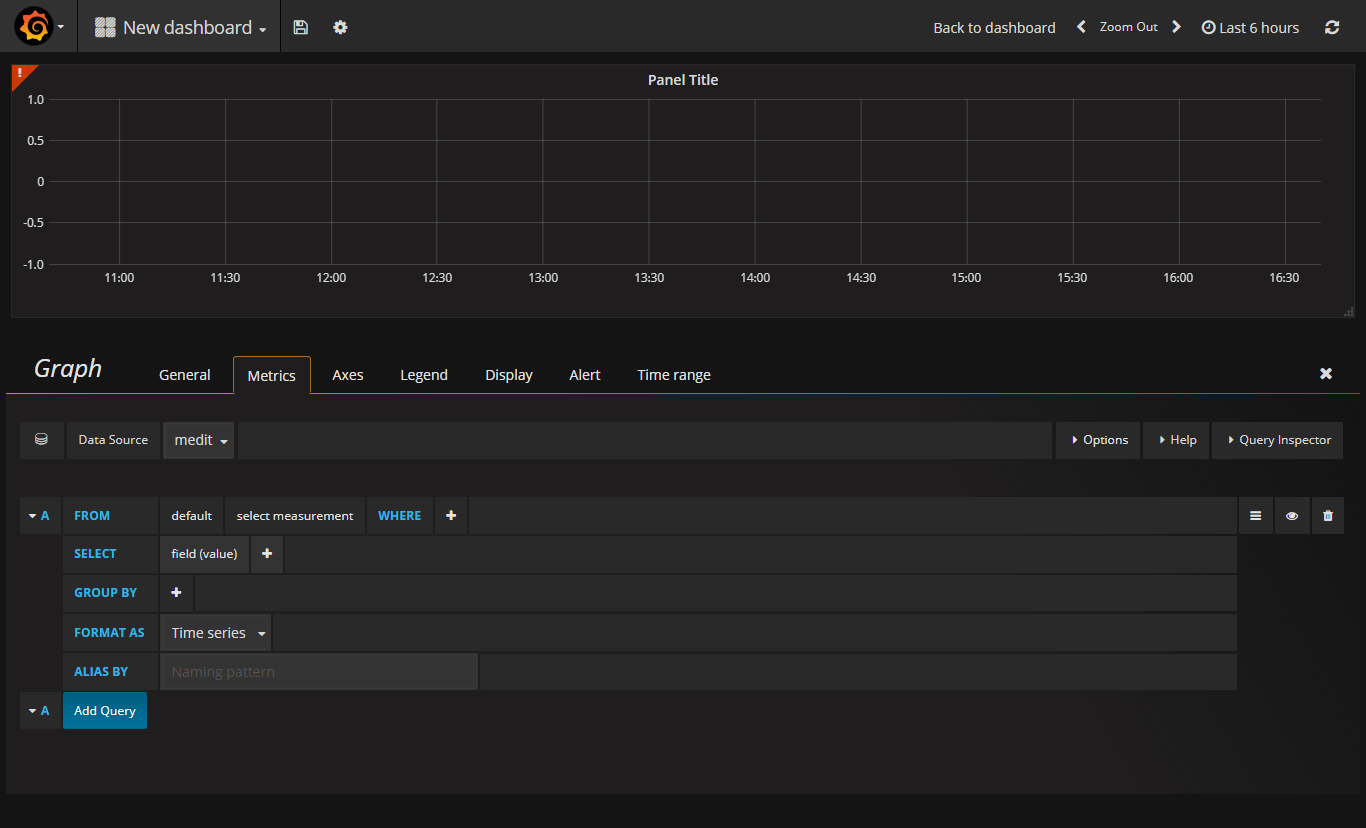
\includegraphics[width=16cm,height=15cm,keepaspectratio=true]{images/gr_query}
	\caption{
		Interface to add query for the panel.
	}
	\label{fig:gr_query}
\end{figure}


\section{Lambda Architecture for Big Data Processing} \label{sec:lmb_arc}
The amount of data being processed nowadays is enormous, and this is often coined as ``Big Data''. Big data can be found everywhere in the form of weblogs, events, social networks, and sensor data, and these all are generating around petabytes of data each day. And because of this huge amount of data, the traditional tools and storage technologies are unable to handle and cope with it. Therefore, this has led to a technology phase shift on how we keep and manage our data, and to the development of advance analytics solutions.

Lambda architecture \cite{UBDLAH}, \cite{oreillyla}, \cite{7364082}, \cite{maprla} is getting involved in machine learning and data science applications by enabling the real-time data processing and analytics without using the traditional extract, transform, load (ETL) approach. It is designed to address the fault-tolerance, scalability and robustness issues of big data systems. Moreover, lambda architecture also ensures the low latency and accuracy of the result. It combines the power of stream processing with batch processing in the system.
Lambda architecture, as shown in Figure \ref{fig:lambda_arc}, consists of 3 main components:

\begin{figure}[htpb]
	\centering
	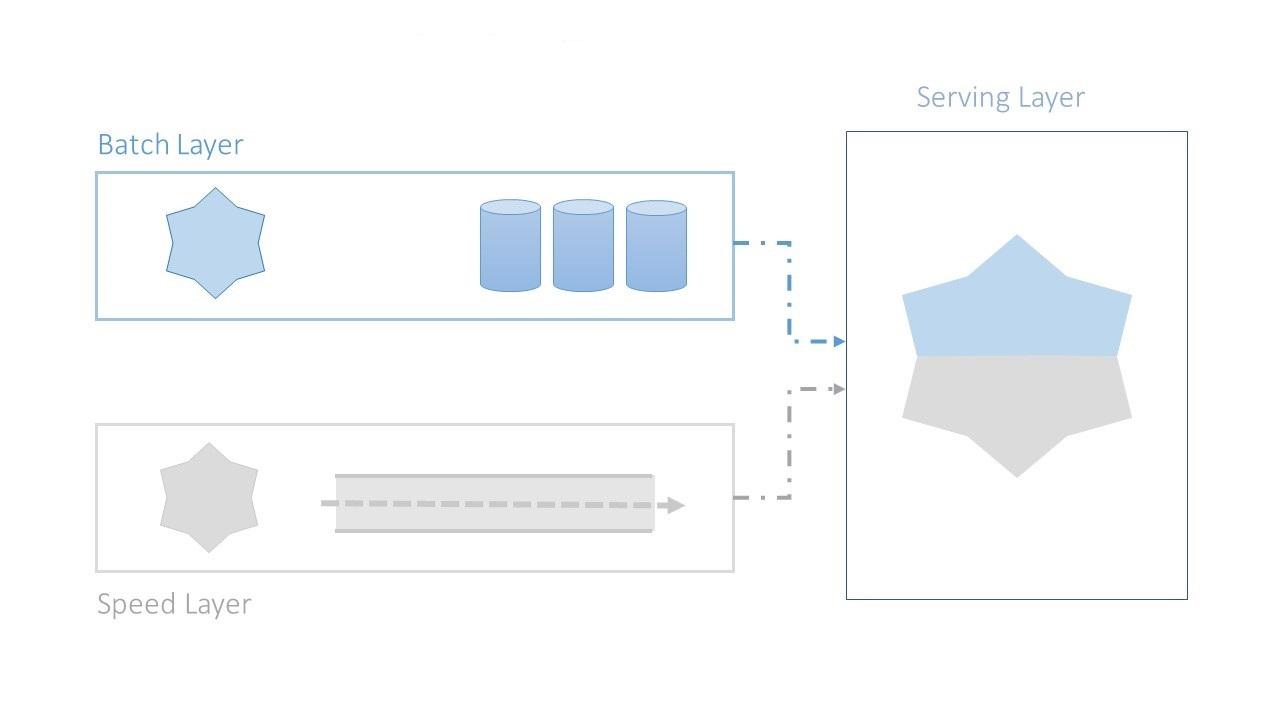
\includegraphics[width=12cm,height=10cm,keepaspectratio=true]{images/lambda_arc}
	\caption{
		Lambda architecture.
	}
	\label{fig:lambda_arc}
\end{figure}



\subsection{Batch Layer}
The batch layer holds all of the master data, which is stored in Apache Hadoop. This data is kept in its original state, untouched and in an immutable manner. This data is processed and generates the batch views, which are served in the serving layer. The batch view provides the most accurate results from the data using one of the available distributed platform tools.

\subsection{Speed Layer}
Typically, it is known that Hadoop processing frameworks are slow and take a lot of time. To cope with this problem, lambda architecture introduces a speed layer. Speed layer processes the real-time stream and generates the real-time views of a short time frame, which is then served as a serving layer along with batch views. The main point to notice here is that the speed layer data is temporal in nature, i.e. it can only store that much amount of data in the memory. And it is deleted as soon as one batch process is completed.

\subsection{Serving Layer}
This is a place where the final results and data are visualized. Serving layer provides an interface, which integrates real-time views with batch views and unified them together. An accurate view of data will be presented by the batch layer, whereas the fresh view of the data will be presented by the speed layer. It also supports ad-hoc queries, which are optimized for low latency. Tools that can be used in this layers are Cassandra and HBase.

The data source provides the data, which is streamed in the speed layer and at the same time to the batch layer. A batch layer holds the data for a long time and stream layer processes the stream in a window of short time and then provides the calculated result. The serving layer combines the data received from the batch layer, more specifically the batch views, and the data received from the speed layer, and allow them to query from a single interface. The advantage of the lambda architecture is that if one layer is down, the other layer can be used to make the system available. For example, if a speed layer is down, which can happen in the production environment, The batch layer can be used to compensate the failure.

The reason why it is called lambda architecture is that the lambda symbol splits into two parts, which in case of this architecture represents the batch layer and the speed layer. 

\begin{figure}[htpb]
	\centering
	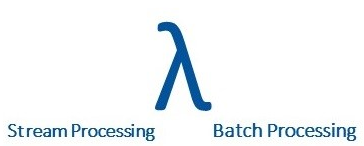
\includegraphics[width=12cm,height=10cm,keepaspectratio=true]{images/lambda_new}
	\caption{
		Lambda symbol representing the lambda architecture.
	}
	\label{fig:lambda}
\end{figure}

Typically, the data stream is implemented using a published and subscribed messaging system such as Apache Kafka, which can easily scale for high-velocity data ingestion. It can be thought of as a place where publishers publish their data and the consumers read data from it. This is different from the traditional queue as it keeps the data until we let it hold. In contrast, the data is removed from the queue, once it is delivered to the appropriate consumer of the data. It uses topics to publish and to subscribe to the data. Every Apache Kafka server is known as a broker and since it is a distributed system, therefore, there can be more than one broker. The more the number of brokers, the higher the availability of the system. The advantage of Apache Kafka is the ability to handle many different forms of data, such as sensors data, application events, server logs, and social network events. Apache Kafka is very fast despite having a heavy load.

\begin{figure}[htpb]
	\centering
	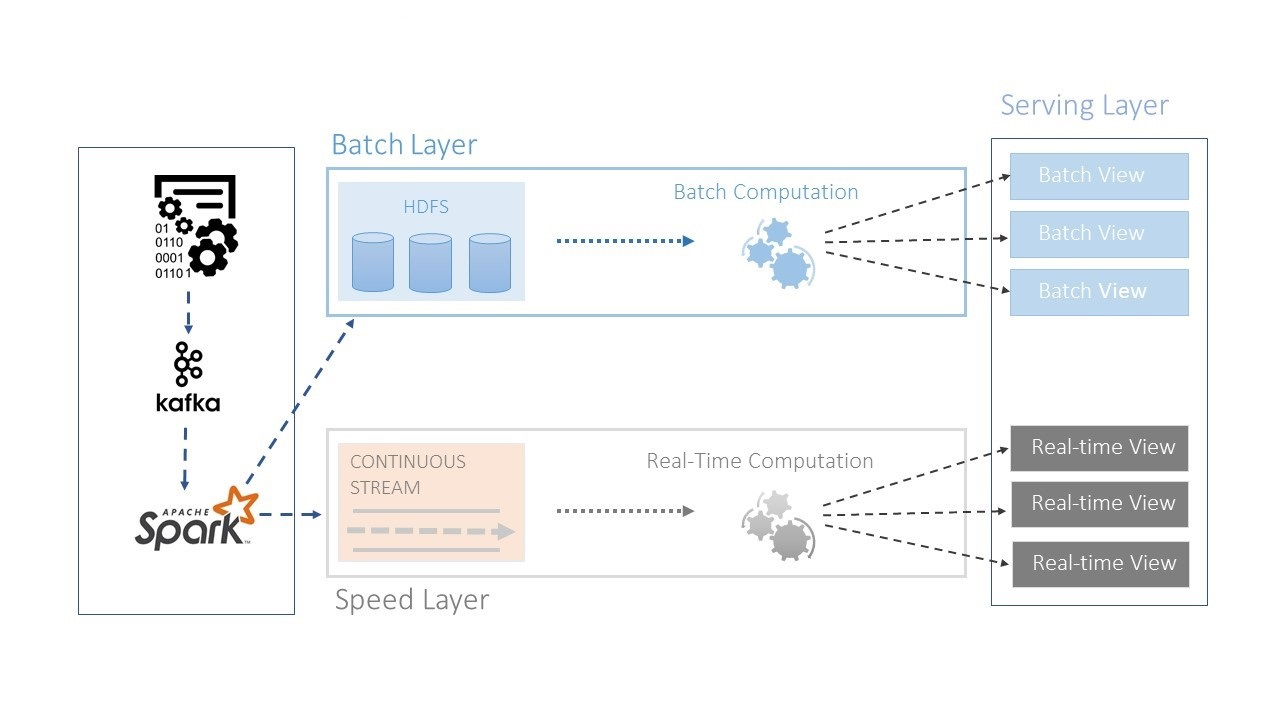
\includegraphics[width=17cm,height=15cm,keepaspectratio=true]{images/imp_lambda_arc}
	\caption{
		Implementation of lambda architecture.
	}
	\label{fig:impl_lambda_arc}
\end{figure}


The implementation of lambda architecture is shown in Figure \ref{fig:impl_lambda_arc}. The data is directly published from the data source to Kafka based on some topic. Data from multiple data sources can be collected via Kafka based on different topic names. Once the data is fed into Apache Kafka, the corresponding consumers will read the data from Apache Kafka using the topic name. In this architecture, Apache Spark can be used in both the batch layer and the speed layer. 

Apache Spark is a large-scale data processing tool. It runs 100 times faster than Apache Hadoop by caching the data objects in the memory. It is fault tolerance as it creates a lineage graph. So, in case of failure, it can do the computations again and go back to the last state of the data. These are two of the fundamental things that Resilient Distributed Data Set (RDD) is all about. It is specially designed to schedule and execute a large amount of data. Apache Spark does not only provide the batch processing, but also provides real-time stream processing, machine learning tools, graph processing, Spark SQL, Spark R and complex analytics. It is designed to run everywhere, such as it can run on Hadoop YARN, Apache Mesos or standalone as well. Apache Spark offers an interface for several programming languages to write the applications. The available languages are for example Java, Scala, Python, and R.


\begin{figure}[h]
	\centering
	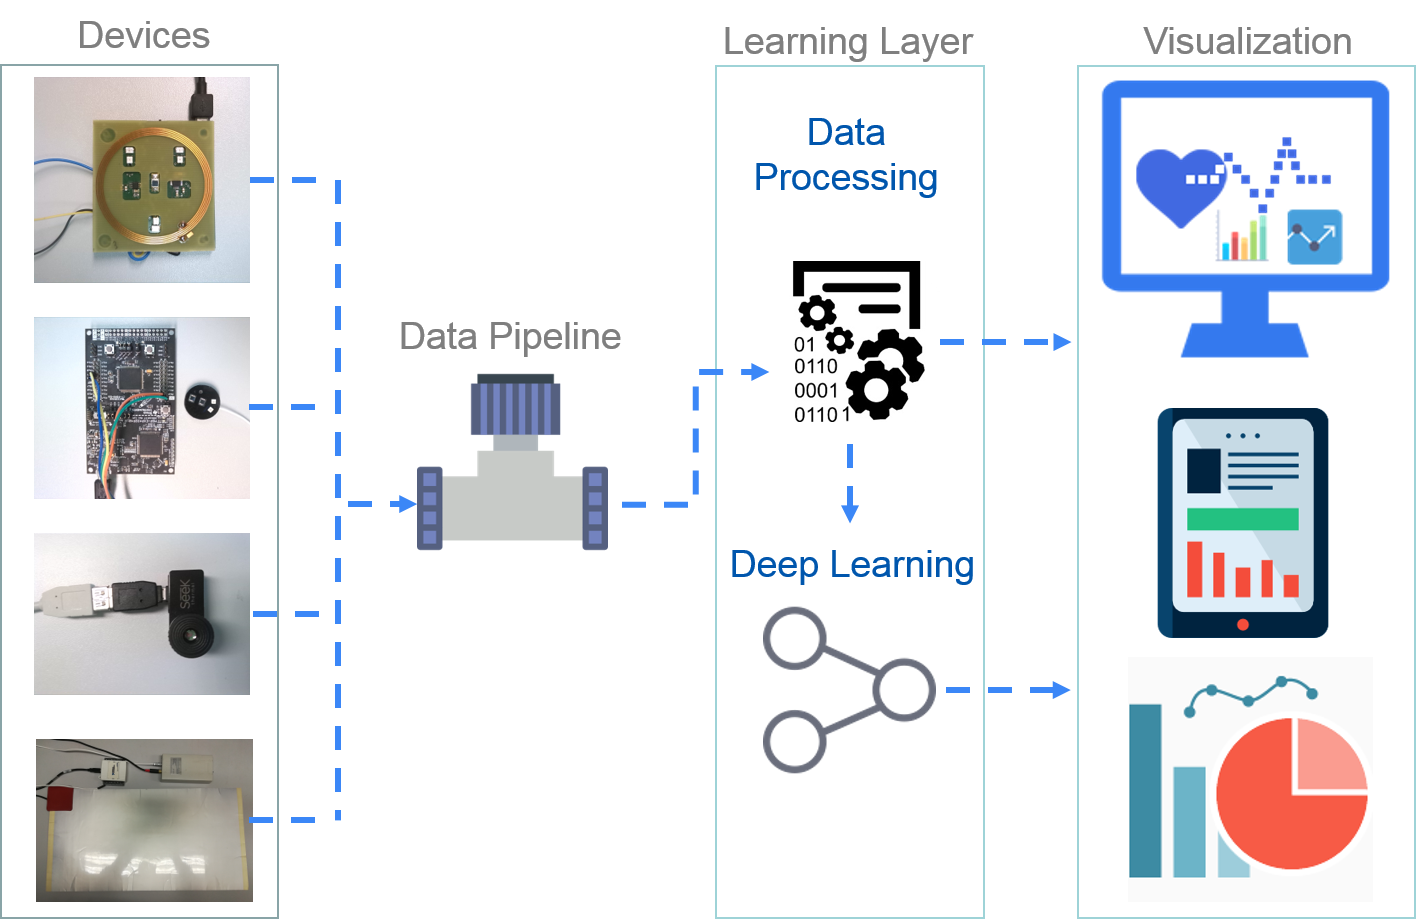
\includegraphics[width=16cm,height=15cm,keepaspectratio=true]{images/sys_arc}
	\caption{
		System architecture for the sensors.
	}
	\label{fig:sys_arc}
\end{figure}

\section{System Architecture}
A system has been implemented to collect, process and visualize the data of all the sensors based on the lambda architecture described in Section \ref{sec:lmb_arc}. But the architecture has been modified because of the lack of enough resources to run all the big data tools.

Batch layer is used for querying over the large dataset to view the result over a long period of time. It is slow and time consuming, and it is not required in our scenario, as we are only interested in the recent data. Therefore, the batch layer has been removed the architecture.

 The modified system architecture can be seen in Figure \ref{fig:sys_arc}. The Python programming language has been used for the system implementation.

The architecture contains 3 main layers:

\subsection{Data Layer}
The data layer contains all the sensors, which generate data in real-time. The data are collected via data pipeline based on their protocol and submit to the speed layer. The data are also immediately stored in InfluxDB in order to have the original state of the data.

\begin{figure}[htpb]
	\centering
	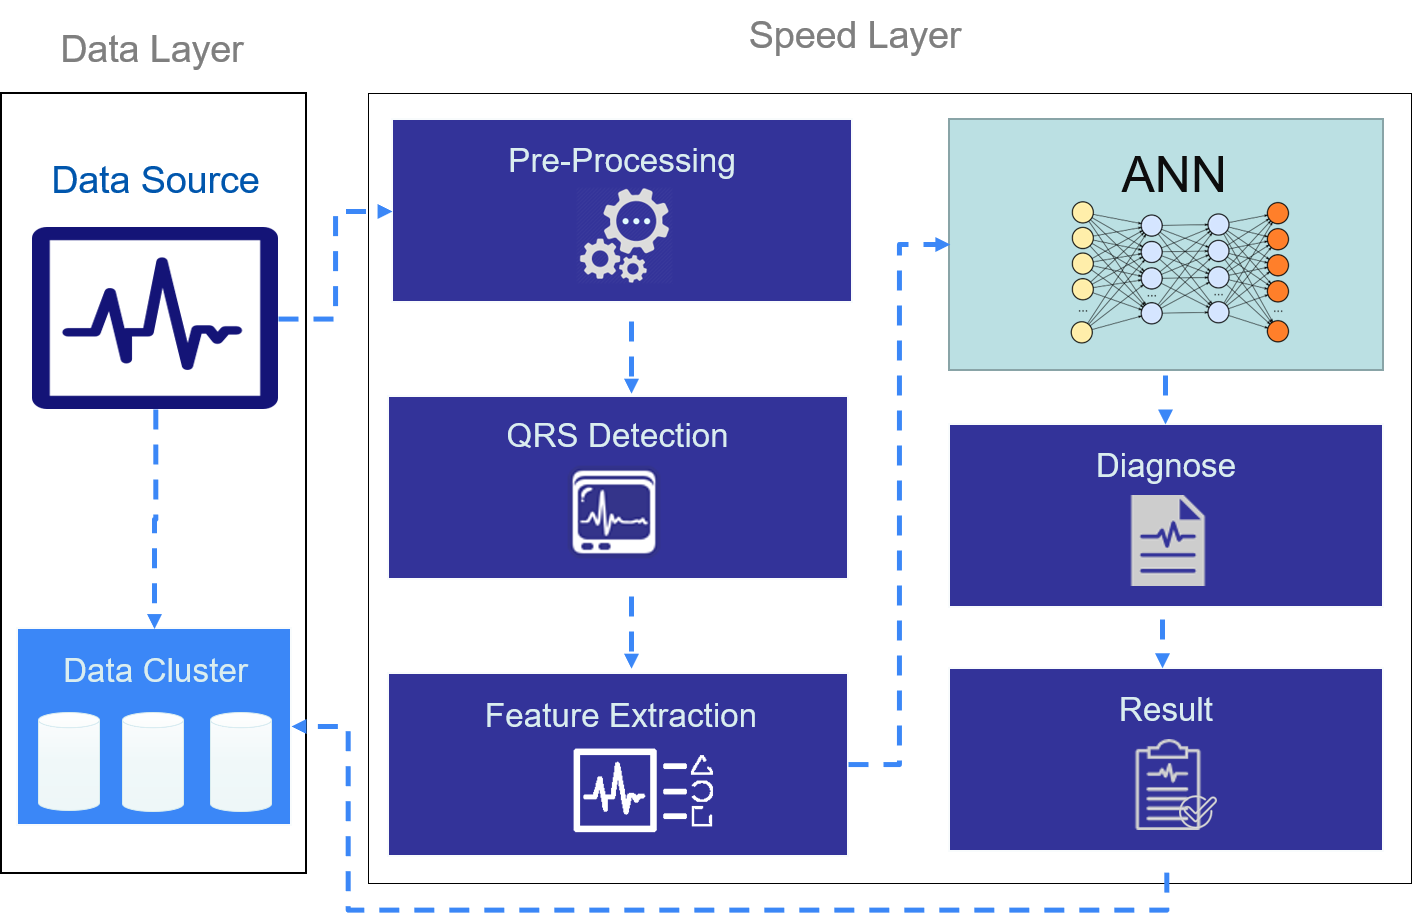
\includegraphics[width=16cm,height=15cm,keepaspectratio=true]{images/ann_usage_speed_layer.png}
	\caption{
		Using the deep learning model in real-time environment.
	}
	\label{fig:using_ann}
\end{figure}


The NI USB-6259 is used for the ECG and BCG signal acquisition. The sampling rate of 360 Hz has been used for ECG signal. The PPG and MI data are collected via serial COM ports.

\subsection{Speed Layer}
The speed layer is the heart of the architecture, where all data are processed and classified by the CNN model. The ECG sensor data is first cleaned and the features are extracted. The algorithm is used that is defined in Section \ref{sec:ecg_det}. Once the R peaks are detected, the single ECG signal corresponding to that R peak, consisting of P, Q, R, S and T peaks is extracted one by one, which is then passed to the deep learning model for the classification of arrhythmia. The other vital signs are also calculated such as heart rate and temperature. The processed signals and the vital signs are also stored in the InfluxDB. The detail view of speed layer is shown in Figure \ref{fig:using_ann}.

\subsection{Serving Layer}
The serving layer allows the sensor signals and vital signs to be visualized. Grafana and android tablets are used for the visualization. Grafana retrieves the desired data from InfluxDB and displays it on the dashboard. Grafana provides many other options such as the refresh time. It specifies how much time query is required for the new data. 

The Grafana selectable dashboards for ECG, MI and PPG sensors can be seen in Figure \ref{fig:ecg_dsh}, \ref{fig:mi_dsh} and \ref{fig:ppg_dsh} respectively.


\begin{figure}[htpb]
	\centering
	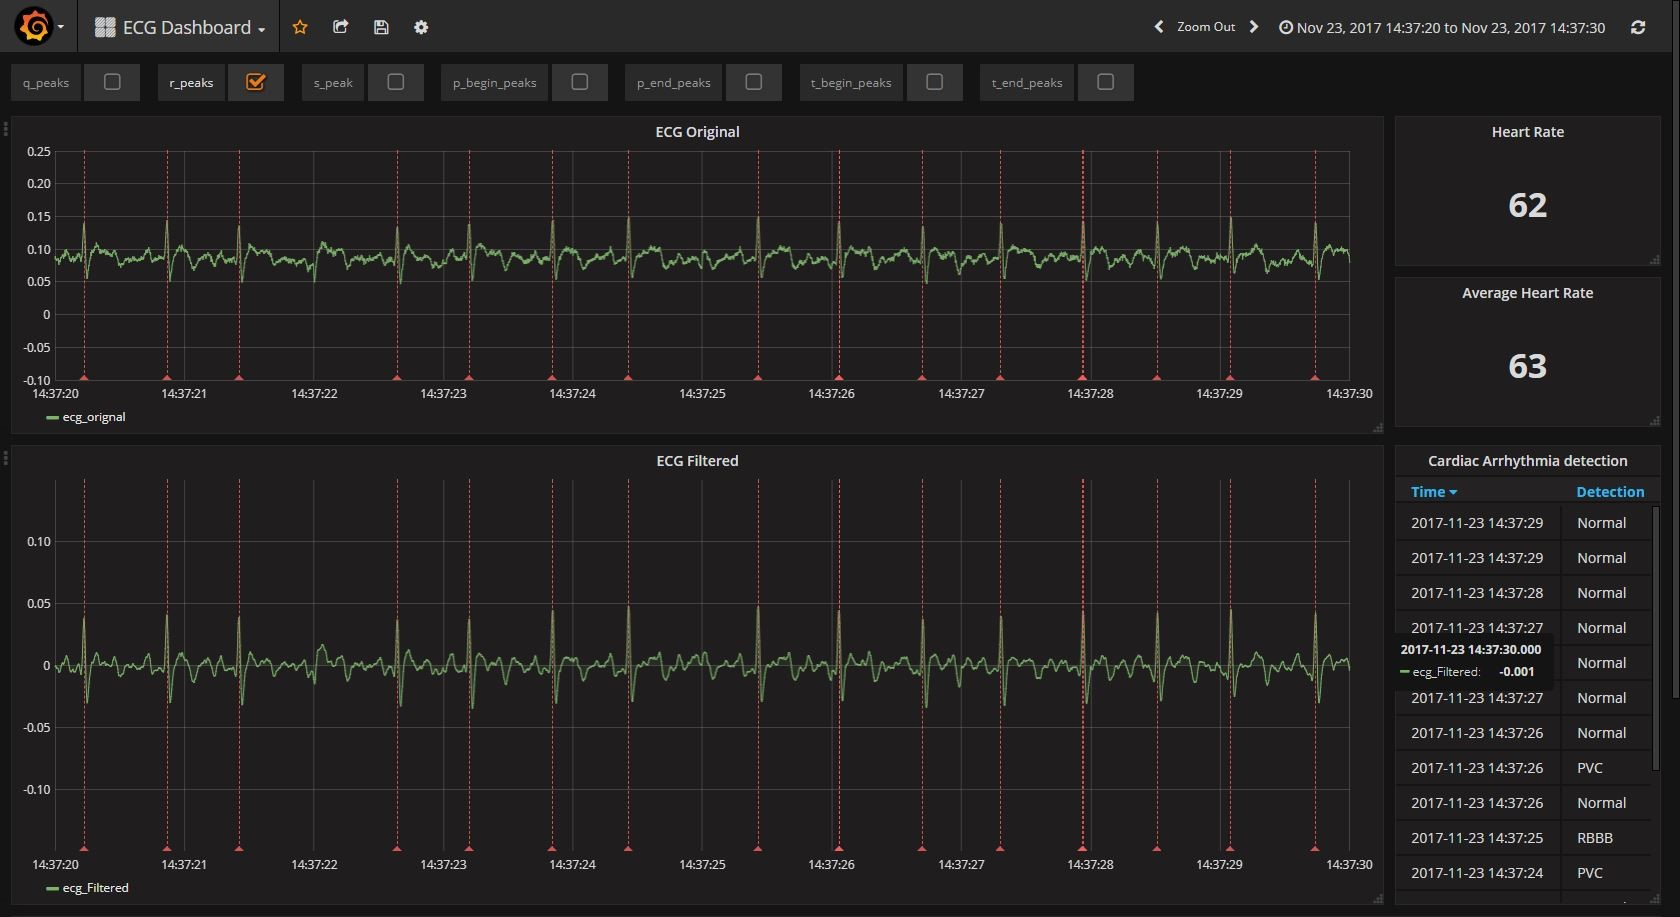
\includegraphics[width=16cm,height=15cm,keepaspectratio=true]{images/ecg_dsh}
	\caption{
		Real-time ECG signal visualization.
	}
	\label{fig:ecg_dsh}
\end{figure}

\begin{figure}[htpb]
	\centering
	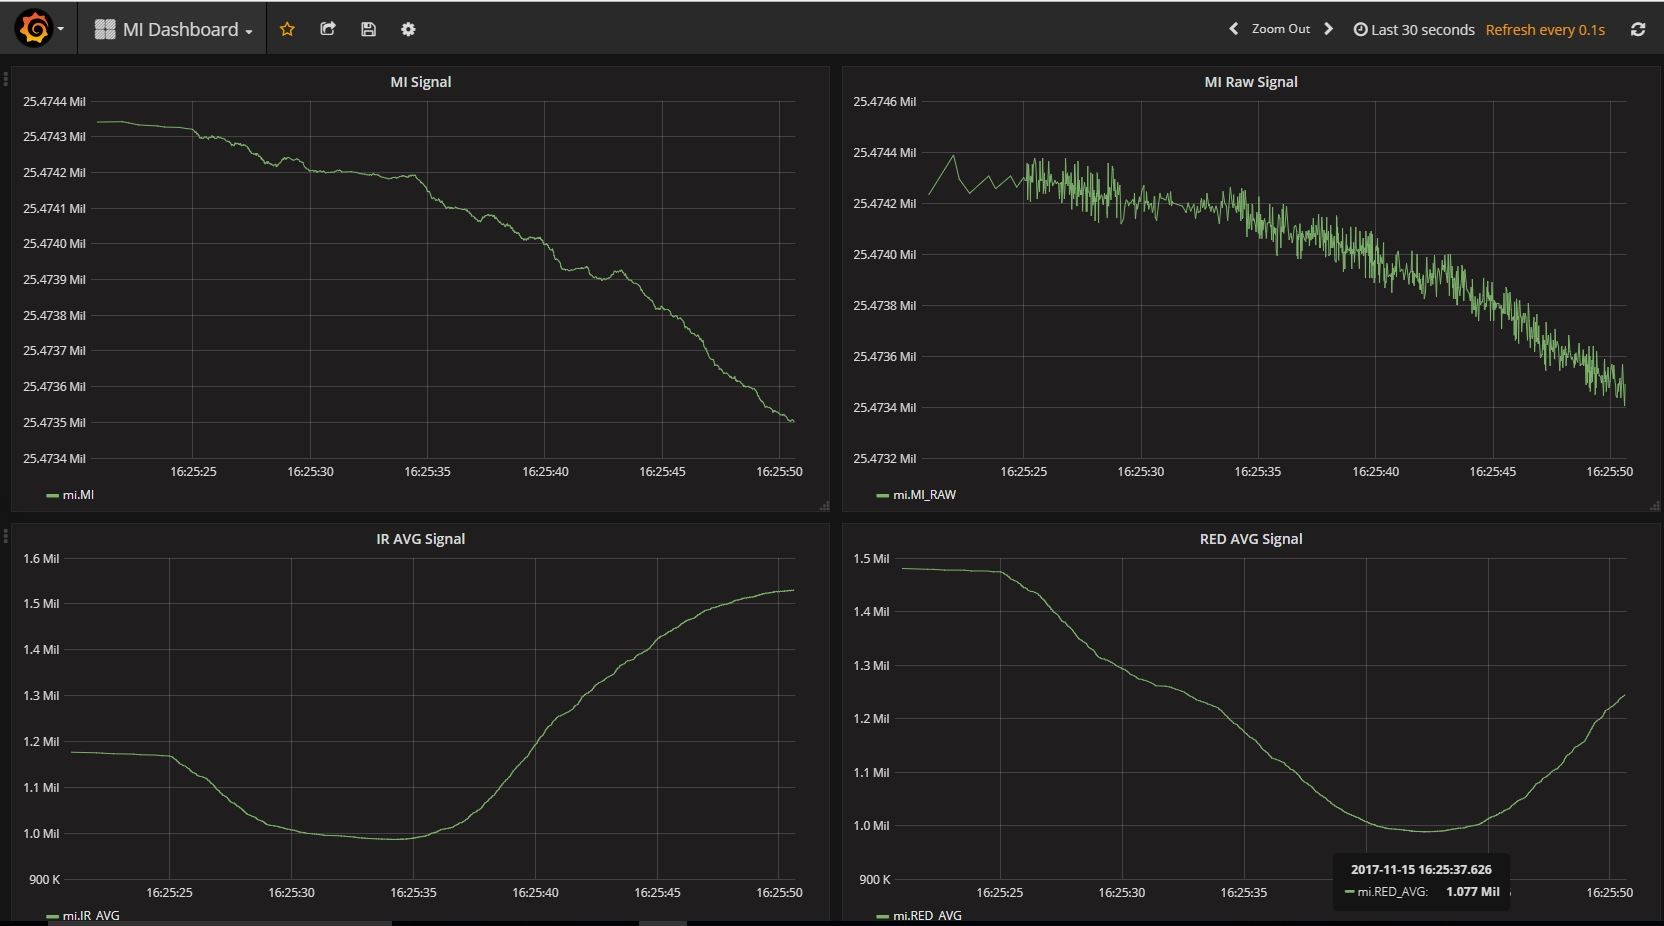
\includegraphics[width=16cm,height=15cm,keepaspectratio=true]{images/mi_dsh}
	\caption{
		Real-time MI signal visualization.
	}
	\label{fig:mi_dsh}
\end{figure}

\begin{figure}[htpb]
	\centering
	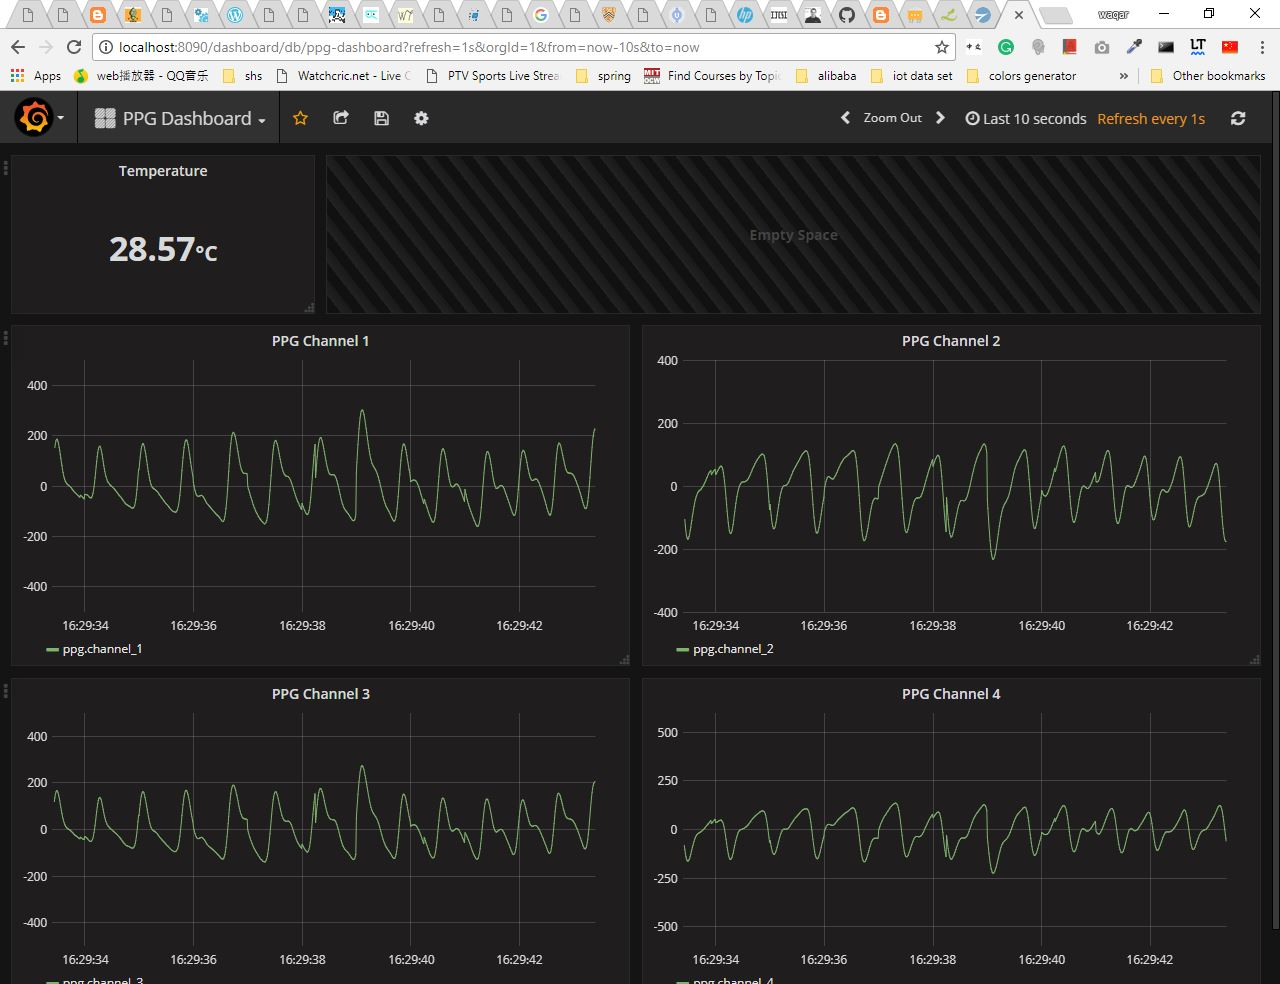
\includegraphics[width=16cm,height=15cm,keepaspectratio=true]{images/ppg_dsh}
	\caption{
		Real-time PPG signal visualization.
	}
	\label{fig:ppg_dsh}
\end{figure}


\subsubsection{Android Application}
An android application has been implemented so that the sensors data can be visualized directly on a mobile device as well. The advantage of the tablet is lightweight with no dependency for data visualization. The screenshot of an Android application can be seen in Figure \ref{fig:ecg_and}.

\begin{figure}[htpb]
	\centering
	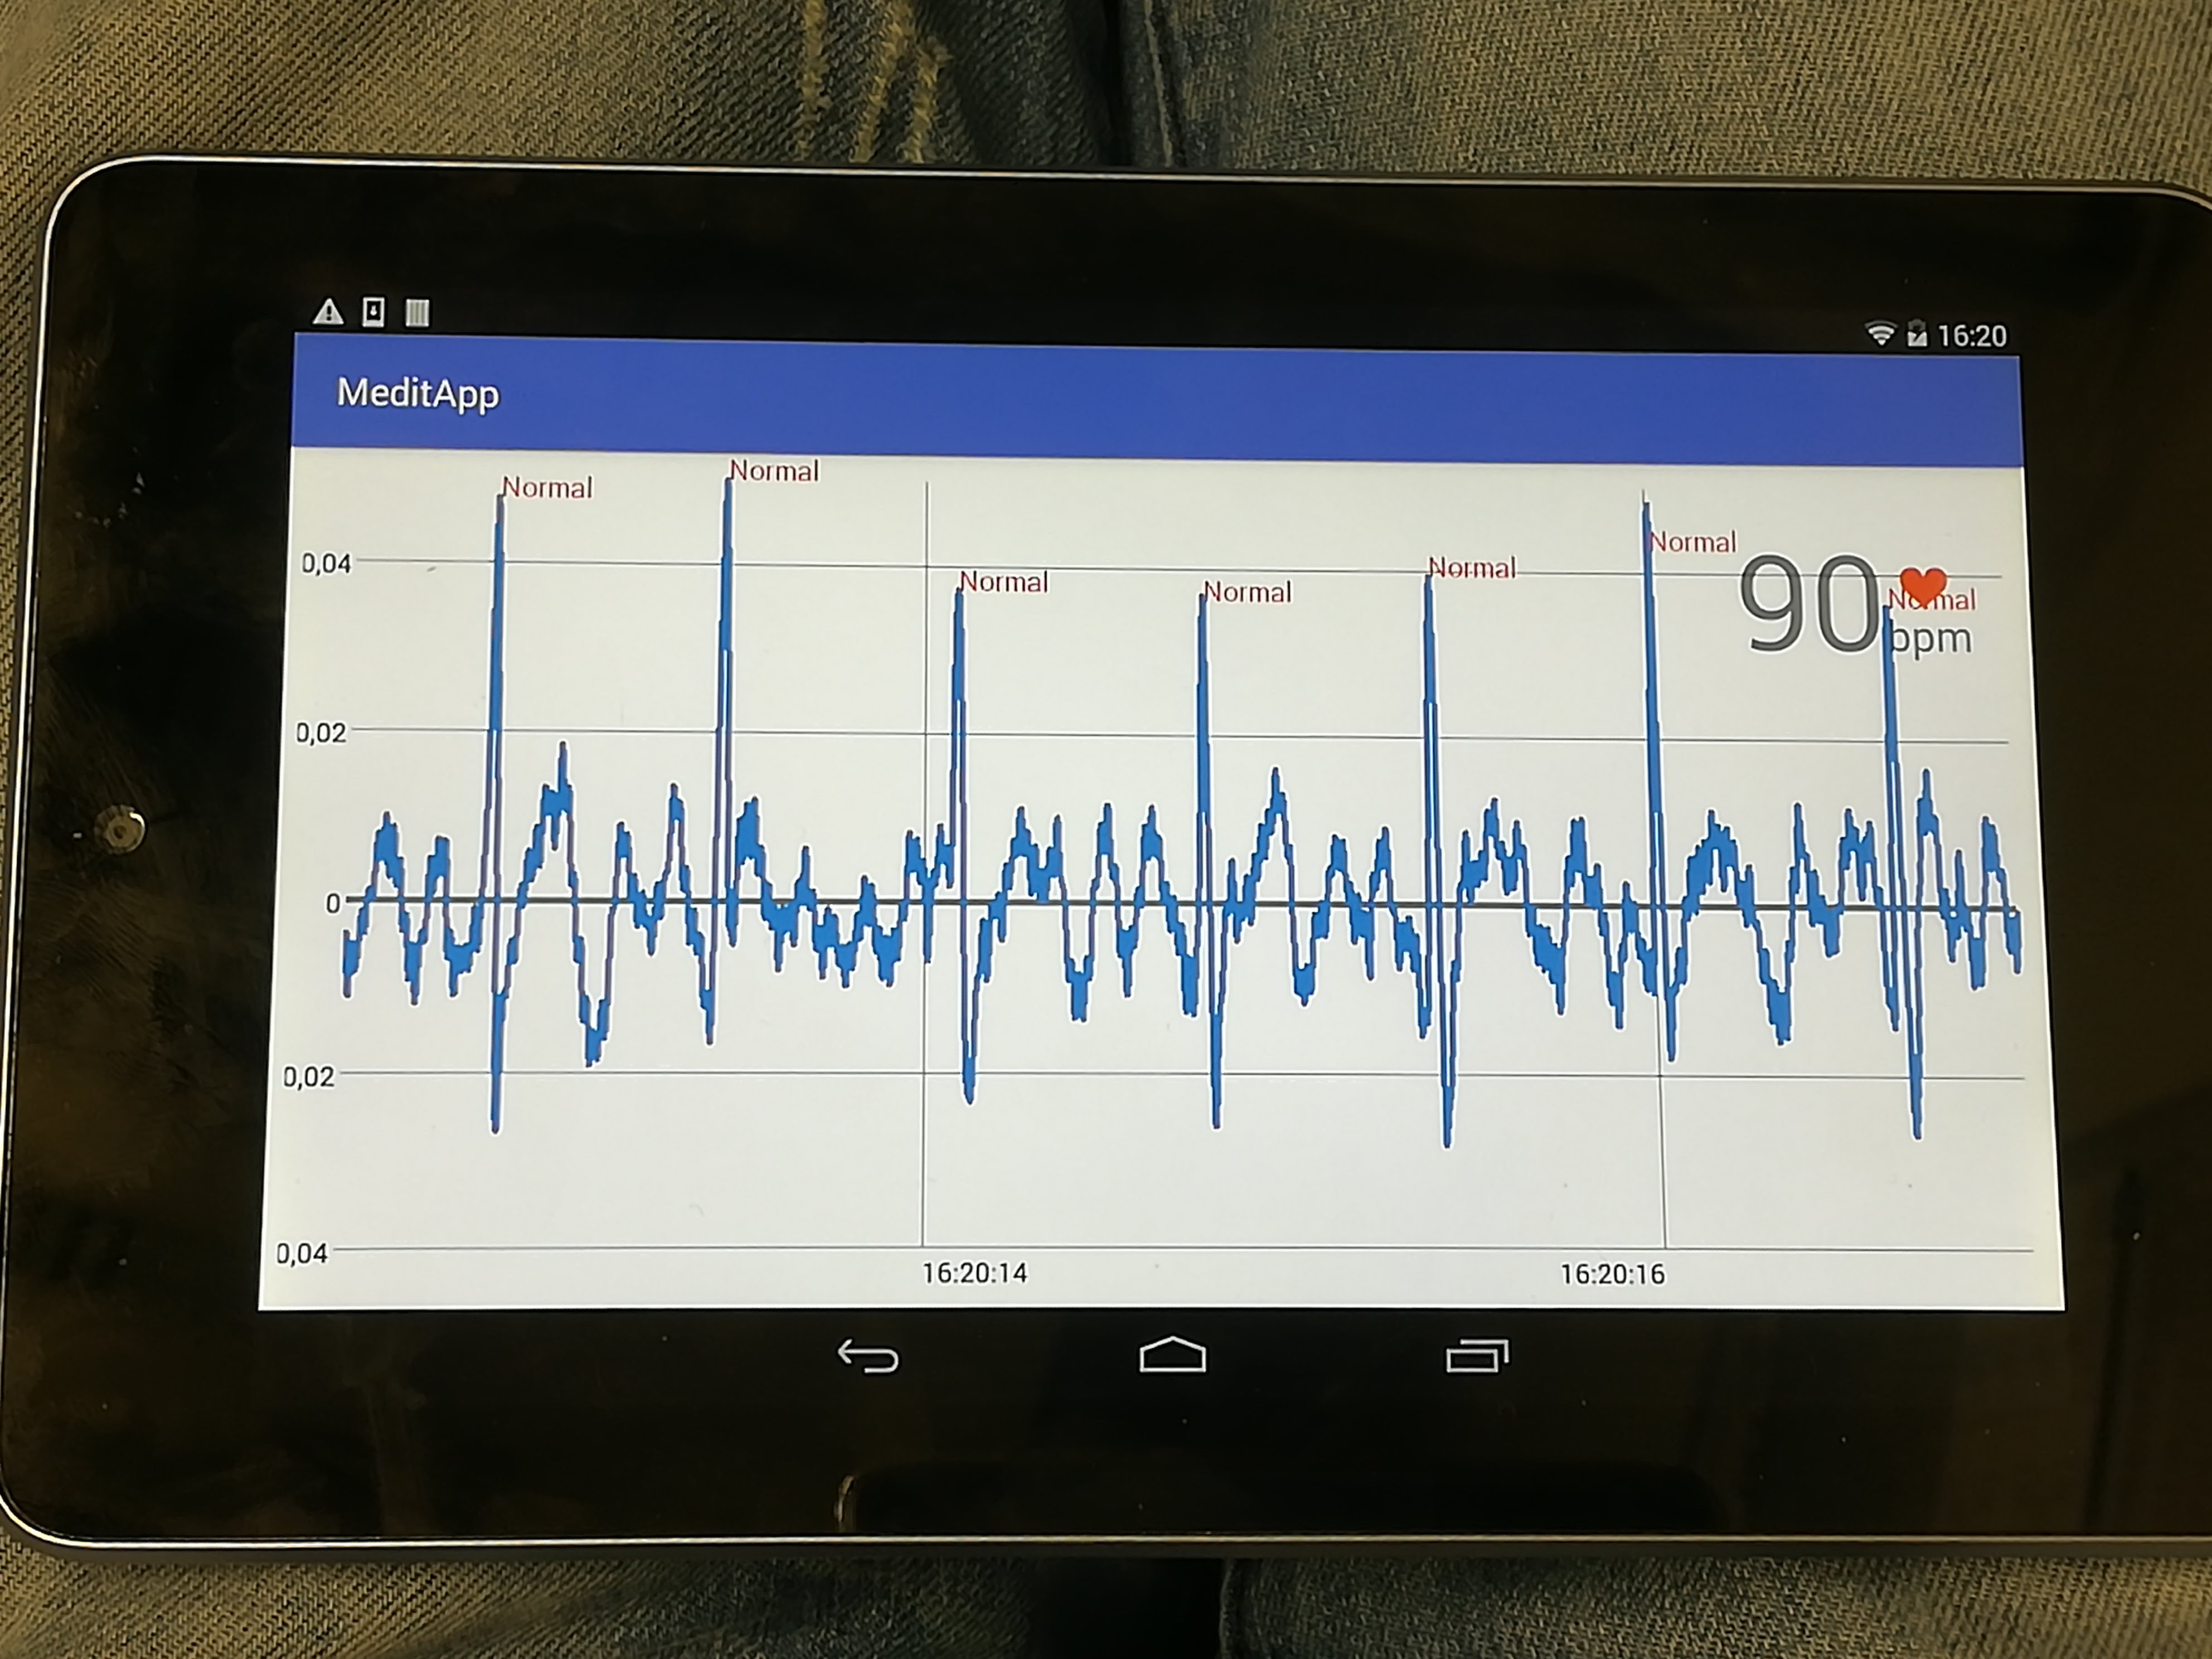
\includegraphics[width=16cm,height=15cm,keepaspectratio=true]{images/ecg_and}
	\caption{
		Real-time ECG signal visualization on android application.
	}
	\label{fig:ecg_and}
\end{figure}



\section{Device Management Interface}
Operating the system via a console is not convenient way to interact with the devices. Therefore, a simple web view interface has also been made to operate the sensor devices. The devices can be started, stopped and in case of error, the logs can be directly viewed in the same interface. The designed interface is shown in Figure \ref{fig:web_int_dev}.


\begin{figure}%
	\centering
	
	\subfigure[][]{%
		\label{fig:ex3-c}%
		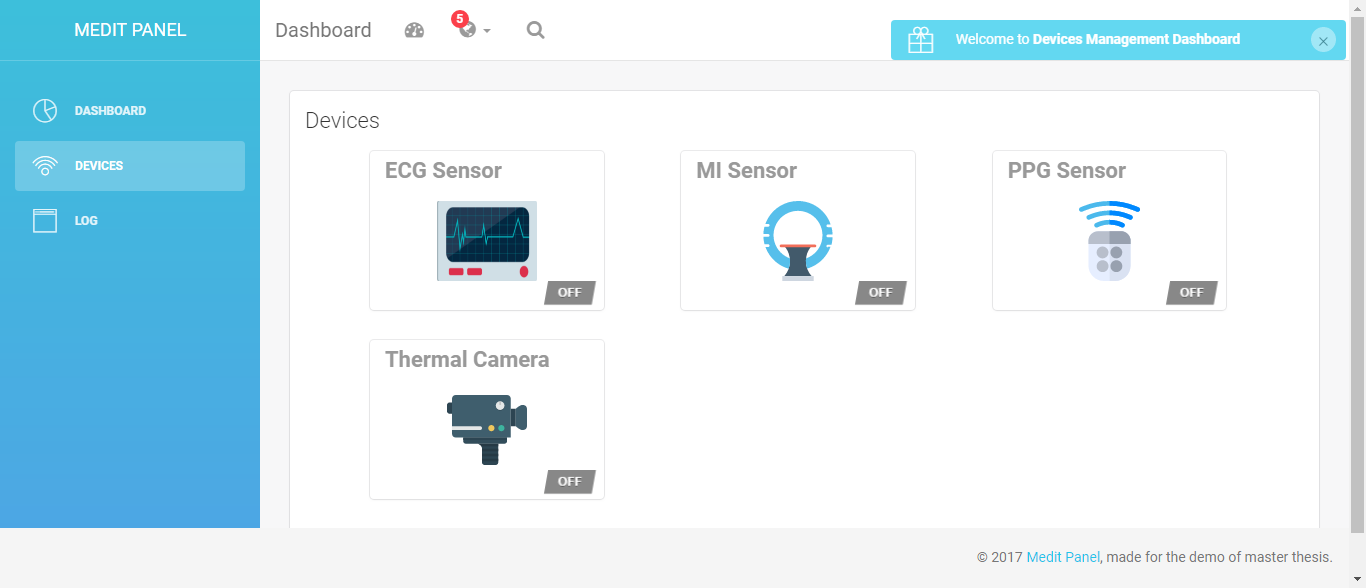
\includegraphics[width=16cm,height=15cm,keepaspectratio=true]{images/medit_dsh_2}}%
	\hspace{15pt}%
	\subfigure[][]{%
		\label{fig:ex3-d}%
		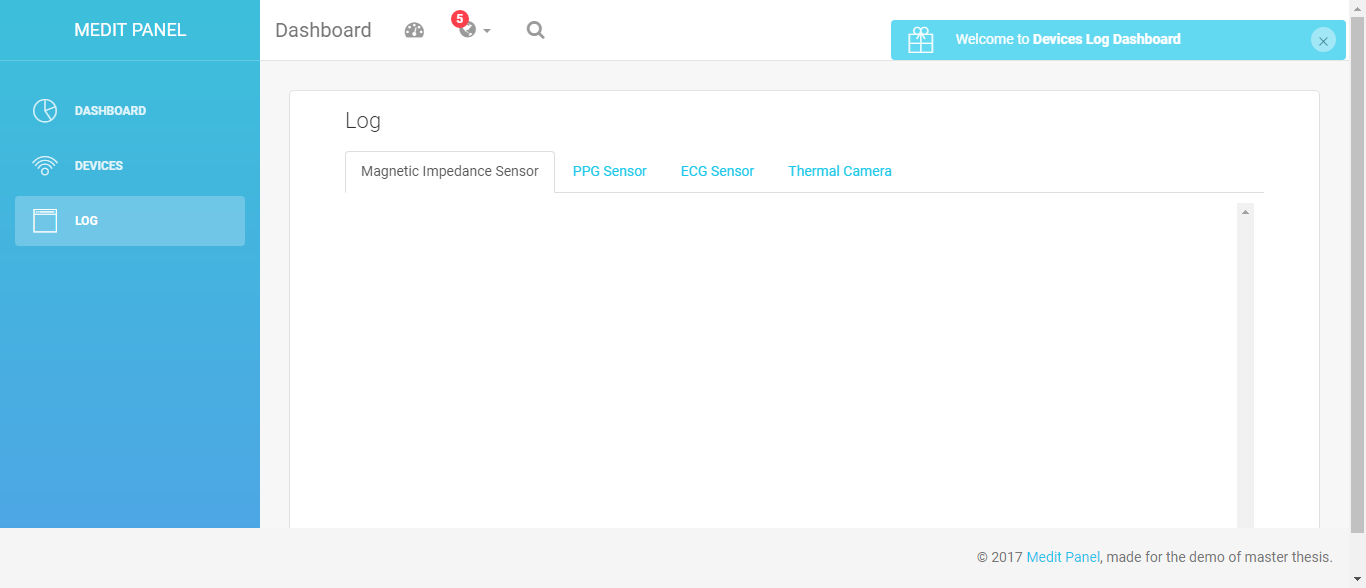
\includegraphics[height=2.7in]{images/medit_dsh_3}}%
	\caption[The device management interface.]{
		\subref{fig:ex3-c} The device management view to interact with devices
		\subref{fig:ex3-d} The log view to represent the state of each device.}%
	\label{fig:web_int_dev}%
\end{figure}
